% Figure from MATH 556 notes, section 34. Compile with the notes preamble.
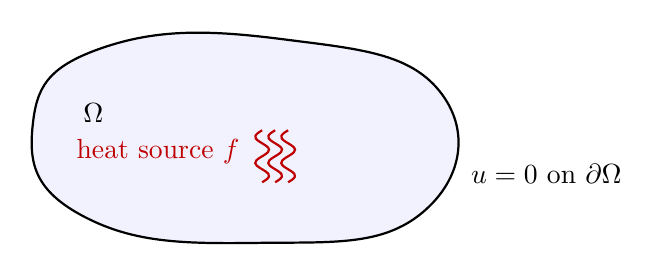
\begin{tikzpicture}[scale=1.1, >=stealth]
    \draw[thick, fill=blue!5] plot[smooth cycle, tension=0.8] coordinates {(-2.4,0.2) (-1.6,1.1) (0.5,1.2) (2.3,0.6) (2.1,-0.8) (0.2,-1.15) (-1.8,-0.85)};
    \node at (-1.7,0.35) {$\Omega$};
    \foreach \dx in {-0.15,0,0.15} {\draw[thick, red!75!black] plot[smooth, domain=0:1, samples=20] ({0.4+\dx+0.08*sin(720*\x)}, {-0.45+0.6*\x});}
    \node[red!75!black, anchor=east] at (0.1,-0.1) {heat source $f$};
    \node[anchor=west] at (2.55,-0.35) {$u = 0$ on $\partial\Omega$};
\end{tikzpicture}
